
\PassOptionsToPackage{subsection=false}{beamerouterthememiniframes}

\documentclass[aspectratio=169]{beamer}
\usepackage[T1]{fontenc}
\usepackage[utf8]{inputenc} 
\usepackage{caption}
\usepackage{lmodern}
\usepackage[french]{babel}
\usepackage{amsmath}
\usepackage{tikz}
\usetikzlibrary{shapes,arrows,automata,positioning}
\usepackage{qtree}
\usepackage{ulem}
\usepackage{pifont}
\usepackage{ragged2e}
\usepackage{fourier-orns}
\usepackage{dsfont}
\usepackage{cancel}
\usepackage{eurosym}
\usepackage{graphicx}
\usepackage[absolute,overlay]{textpos}
\usepackage{wrapfig}
\usepackage{multicol}
\usepackage{bbm}
\usepackage{pdfpages}

\usetheme{Szeged}
\usecolortheme{beaver}

\setbeamertemplate{navigation symbols}{} % suppress the ligne for the navigation bar

\setcounter{tocdepth}{1}

\useoutertheme{miniframes} % Alternatively: miniframes, infolines, split

\definecolor{myred}{RGB}{203,1, 0}
\definecolor{itemred}{RGB}{163,0, 0}
\definecolor{mygray1}{RGB}{236,   236,  236}
\definecolor{mygray2}{RGB}{236,   236,  236}
\setbeamercolor{structure}{fg=itemred} % itemize, enumerate, etc

% alertblock
\setbeamercolor{block title alerted}{fg=myred,bg=mygray2}
\setbeamercolor{block body alerted}{fg=black, bg=mygray1}
\setbeamercolor{frametitle}{bg=mygray2}

\newcommand*\oldmacro{}%
\let\oldmacro\insertshorttitle%
\renewcommand*\insertshorttitle{%
  \oldmacro\hfill%
  \insertframenumber\,/\,\inserttotalframenumber}

\logo{ 
\includegraphics[width=6cm,  keepaspectratio, trim=0cm 12.3cm 26cm 0cm]{logos/logo_chu_uni.png} }


\title[Title of the seminar/congress]{Title of your presentation}

\author{Your name}

\date{Title of the seminar/congress,  City \\ Date}

\AtBeginSection[]
{
 \begin{frame}<beamer>
 \frametitle{Table of contents}
 \tableofcontents[currentsection]
 \end{frame}
}

\begin{document}

\frame{

\thispagestyle{empty}

\titlepage

\begin{figure}
\hspace*{-0.5cm} 
\centering

\includegraphics[width=13cm,  keepaspectratio,  trim=0cm 0cm 2cm 0cm,  clip]{logos/all-logos.png}
\end{figure}
} 


\section{The best sentences}

\frame{

  \frametitle{Star wars or not?}
  
\begin{itemize}

\item Dark vador is not my father.

\item Are you sure Anakin?

\item Yes, my father said:

\begin{itemize}

\item The yes needs the no to win against the no.\footnote{Jean-Pierre Raffarin, Archive INA,https://www.youtube.com/watch?v=O27mdRvR1GY}

\end{itemize}

\end{itemize}
}


\section{More seriously with math and graphs}

\frame{

  \frametitle{The conditions for augmenting Radomized CLinical Trials (RCT) with an external control group \footnote{Dang et al.  A Cross-Validated Targeted Maximum Likelihood Estimator for Data-Adaptive Experiment Selection Applied to the Augmentation of RCT Control Arms with External Data.  arXiv:2210.05802v1}}
  
\begin{itemize}

    \item[C1.] The respect for positivity between the external and RCT controls.
    
    \item[C2.] The absence of unmeasured confounders,  i.e.  determinants of both the  outcome and the probability of inclusion in the RCT compared to the external group.
    
    \item[C3.] The absence of a direct effect on the outcome of being included in the RCT.
    
\end{itemize}
}


\frame{

  \frametitle{How to respect the condition C1 (positivity)?}
  
\begin{enumerate}

    \item Use external data but from a recent period.
    
    \item Use external data from the same centers,  at least for a large part.
    
    \item Check the inclusion criteria in both the RCT and external study: the targeted population of the RCT must be embedded.
    
    \item Compare the characteristics of two samples of controls to validate the positivity, \footnote{Danelian G,  Foucher Y,  Léger  M, Le Borgne F.  and  Chatton A.  Identification of in-sample positivity violations using regression trees: The PoRT algorithm.  Journal of Causal Inference (2023).} and restrict the inclusion criteria until no issue is identified.
    
\end{enumerate}
}


\frame{

  \frametitle{How to respect the condition C2 (absence of unmeasured confounders)?}
  
\begin{enumerate}

    \item Draw a causal diagram with the inclusion in the RCT versus external study as an element.  
    
    \item Propose a complete list of the prognostic factors of the studied outcomes.
    
    \item Propose a complete list of the determinants of the inclusions in the RCT versus external study.
    
    \item Make sure that the variables in the two lists \#2 and \#3 will be available in both the RCT and the external study with the same methods of collection.
   
\end{enumerate}
}


{ \logo{} \frame{

  \frametitle{How to respect the condition C3 (no direct effect of being in the RCT)?}
  
\begin{itemize}

   \item  One can limit/prevent such a direct effect by:
   
\begin{enumerate}

    \item  Check the studied treatments are identical in the two studies (doses, administration,  etc.).
    
    \item  Use the same definition of the collected outcomes.
    
    \item  Ensure comparable monitoring  in the two studies.
    
\end{enumerate}

   \item Control patients in the RCT are required for a data-driven check of C3.
   
   \item  An RCT based on a control arm completely-based with external data or digital twins does not allow for validating C3.
    
\end{itemize}
    
\begin{alertblock}{Problem \#2 : these checks do not convince on the respect of C3}

\begin{itemize}

   \item \textbf{How to validate C3  by using the RCT data?}
    
\end{itemize}
    
\end{alertblock}
} }


{ \logo{} \frame{

\frametitle{Consider the following usual RCT for superiority with k controls for 1 patient in the experimental arm}
  
\begin{itemize}

   \item A binary principal outcome $Y$ with $\pi_0$ and $\pi_1$ the two expected proportions in the control and experimental arms.
   
   \item $N_{1s}$ and $N_{0s}$ the required sample sizes for a bilateral test with targeted type-I and type-II errors, $\alpha$ and $\beta$ respectively.
    
   \item $ N_{0s} = k N_{1s} $ and $ N_{1s} =  ( \pi_1 -  \pi_0 )^2   (    \pi_0 (1 -  \pi_0 )    / k    +  \pi_1(1 -  \pi_1 )  ) / (z_{\alpha / 2} + z_{\beta } )^2  $
   
\end{itemize}
    
\begin{alertblock}{Example}

\begin{itemize}

   \item For $k=1$,  $\alpha=0.05$,  $\beta=0.20$,  $\pi_0=0.50$ and $\pi_1=0.40$,
   
   \item the sample sizes are $ N_{0s} = N_{1s} = 385$.

\end{itemize}
    
\end{alertblock}
}   }
    

    
\frame{

  \frametitle{Consider the following method to augment the RCT with external data (one method among others)}
  
\begin{itemize}

   \item A model $M$ (for instance a logistic regression) is estimated from the external data to predict the outcome $\hat{\pi}_{0i}$ given the characteristics $X_i$ of a patient $i$ with the control treatment.
   
   \item There is no direct effect of being in the RCT (condition C3) if $M$ is well-calibrated for the outcome prediction at the inclusion in the control group of the RCT.
   
   \item A calibration measure can be $O/E$:
   
\begin{itemize}

    \item $O$ is the number of observed events : $ \sum_i Y_i$ among the control patients.
    
    \item $E$ is the number of expected events: $ \sum_i \hat{\pi}_{0i}$ among the control patients.
    
\end{itemize}
    
   \item The value $O/E=1$ indicates a perfect calibration.
   
\end{itemize}
}    
    
    
{ \logo{} \frame{

  \frametitle{Minimal sample size $N_{0c}$ to evaluate the calibration of the model $M$}
  
\begin{itemize}

   \item By using the delta method:\footnote{Debray et al.  A framework for meta-analysis of prediction model studies with binary and time-to-event outcomes. Stat Methods Med Res. 2019;28:2768-2786. }  $SE(\log(O/E) \approx  \sqrt{ (1-\pi_{0} ) / ( \pi_{0}  N_{0c} ) }$. 
   
   \item Depending on $w$,  the targeted width of confidence interval of the O/E,  one can compute $SE_w(\log(O/E)$.
   
   \item  One can deduce that   $ N_{0c}  = (1-\pi_{0} )  / (\pi_{0} SE_w(\log(O/E)^2 )$
   
\end{itemize}
    
\begin{alertblock}{Example (continued,  with $k=1$,  $\alpha=0.05$,  $\beta=0.20$,  $\pi_0=0.50$ and $\pi_1=0.40$)}

\begin{itemize}

   \item For $\alpha=0.05$ and  $w=0.10$ (i.e.,  $SE_w(\log(O/E) \approx 0.25$)  then $ N_{0c} = 1541$. 

\begin{itemize}

   \item   $ N_{0c}  > 385$:  we cannot check the respect of C3.
   
\end{itemize}
   
      \item For $\alpha=0.05$ and  $w=0.20$ (i.e.,  $SE_w(\log(O/E) \approx 0.51$,)  then $ N_{0c} = 386 $. 
      
\begin{itemize}

   \item    $ N_{0c}  \approx  385$:  we can check the respect of C3.
   
\end{itemize}
   
\end{itemize}
    
\end{alertblock}
} }
    
{ \logo{} \frame{

  \frametitle{}
  
\centering
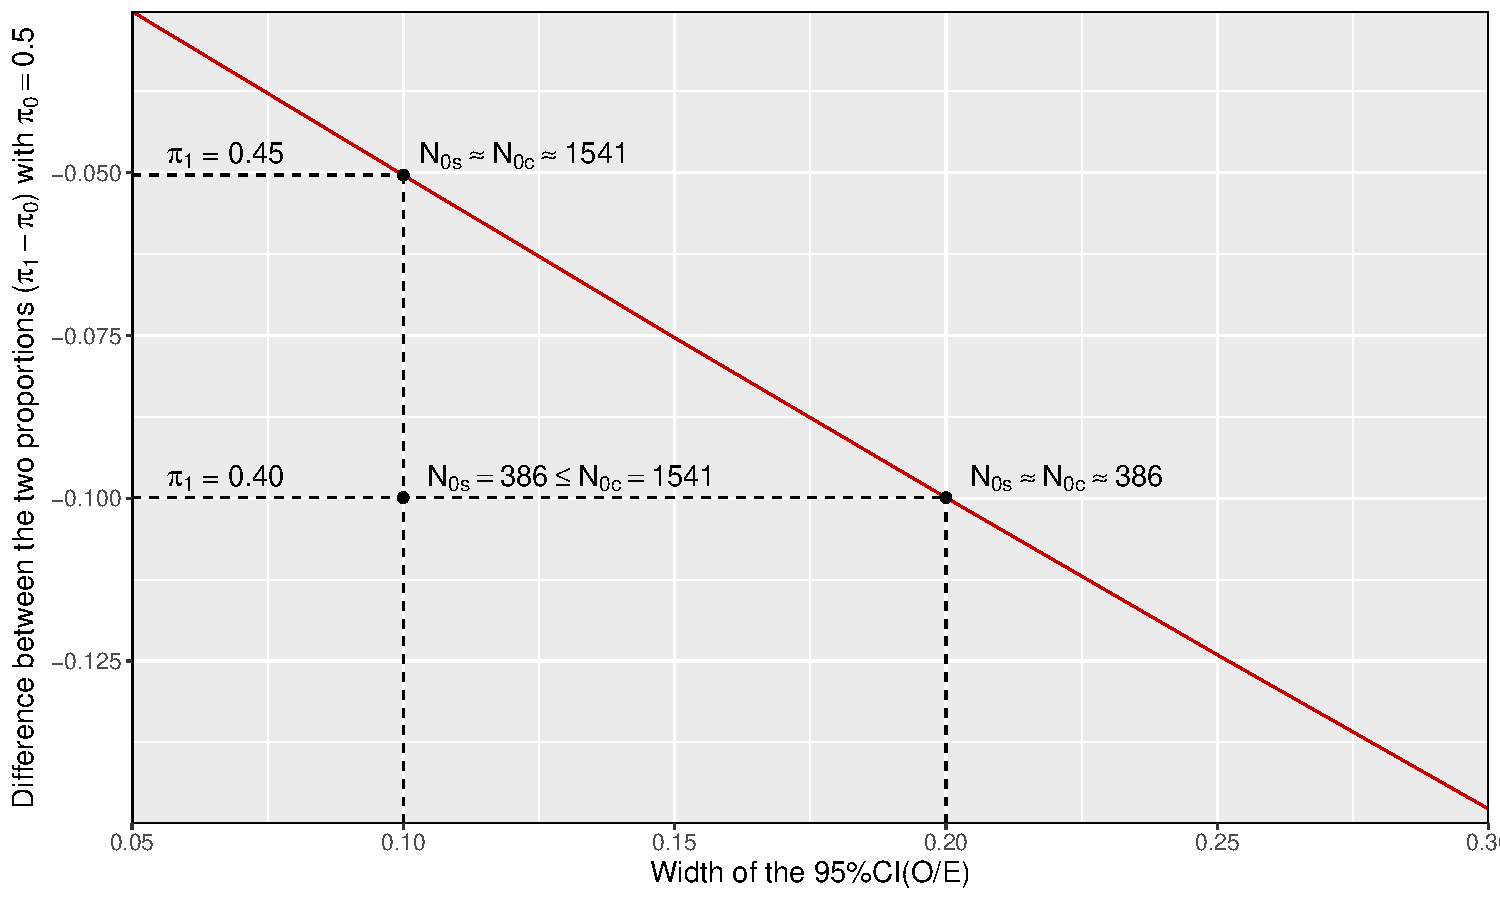
\includegraphics[width=12cm,  keepaspectratio]{figures/ggp1.pdf}
} }

{ \logo{} \frame{

  \frametitle{}
  
\centering
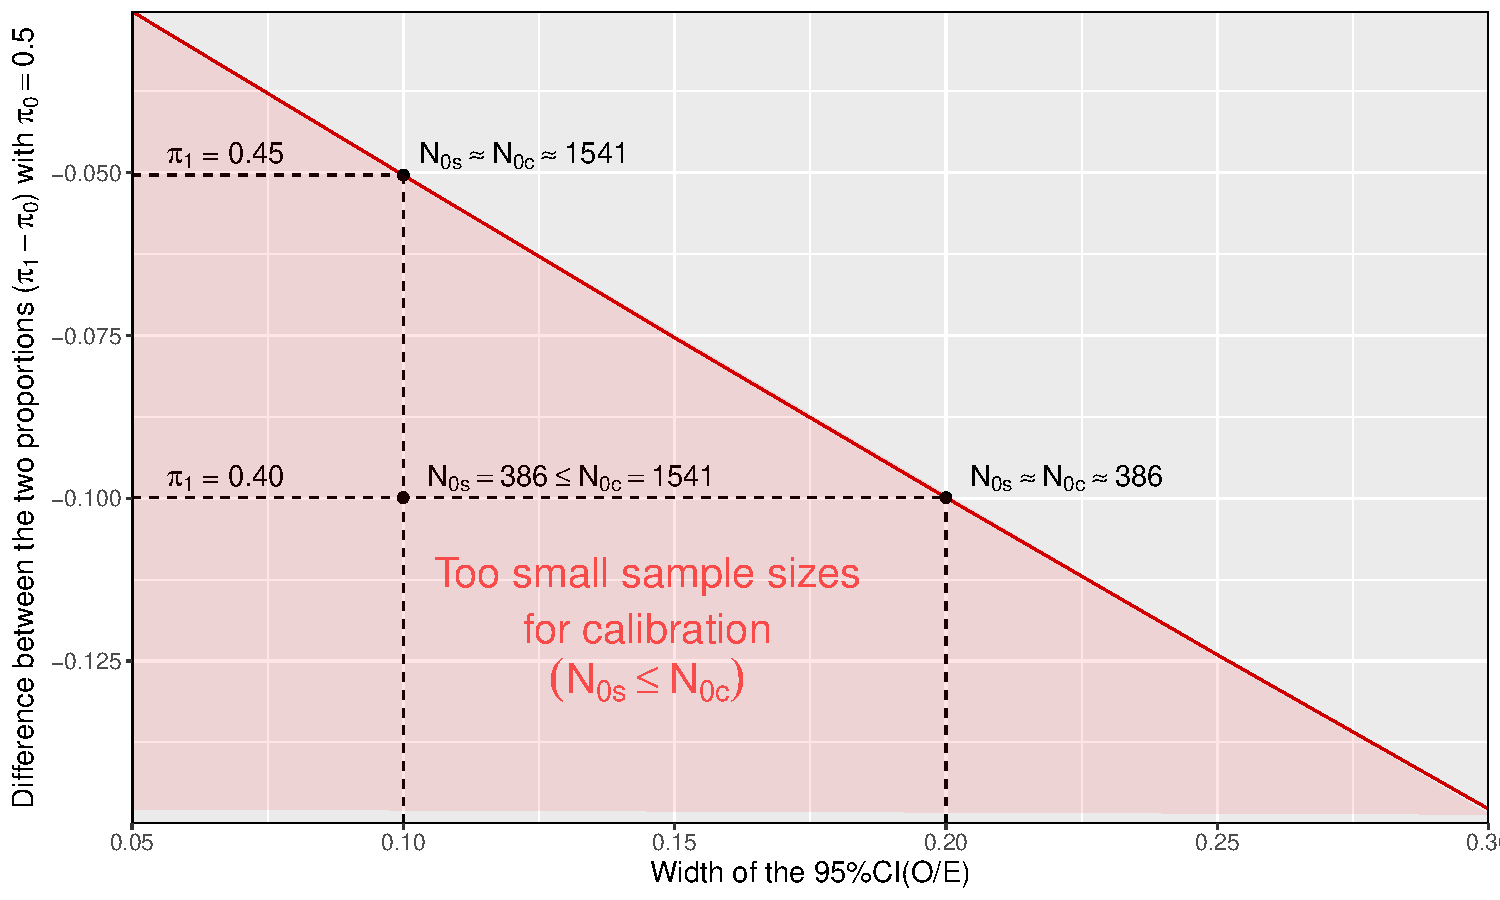
\includegraphics[width=12cm,  keepaspectratio]{figures/ggp2.pdf}
} }

{ \logo{} \frame{

  \frametitle{}
  
\centering
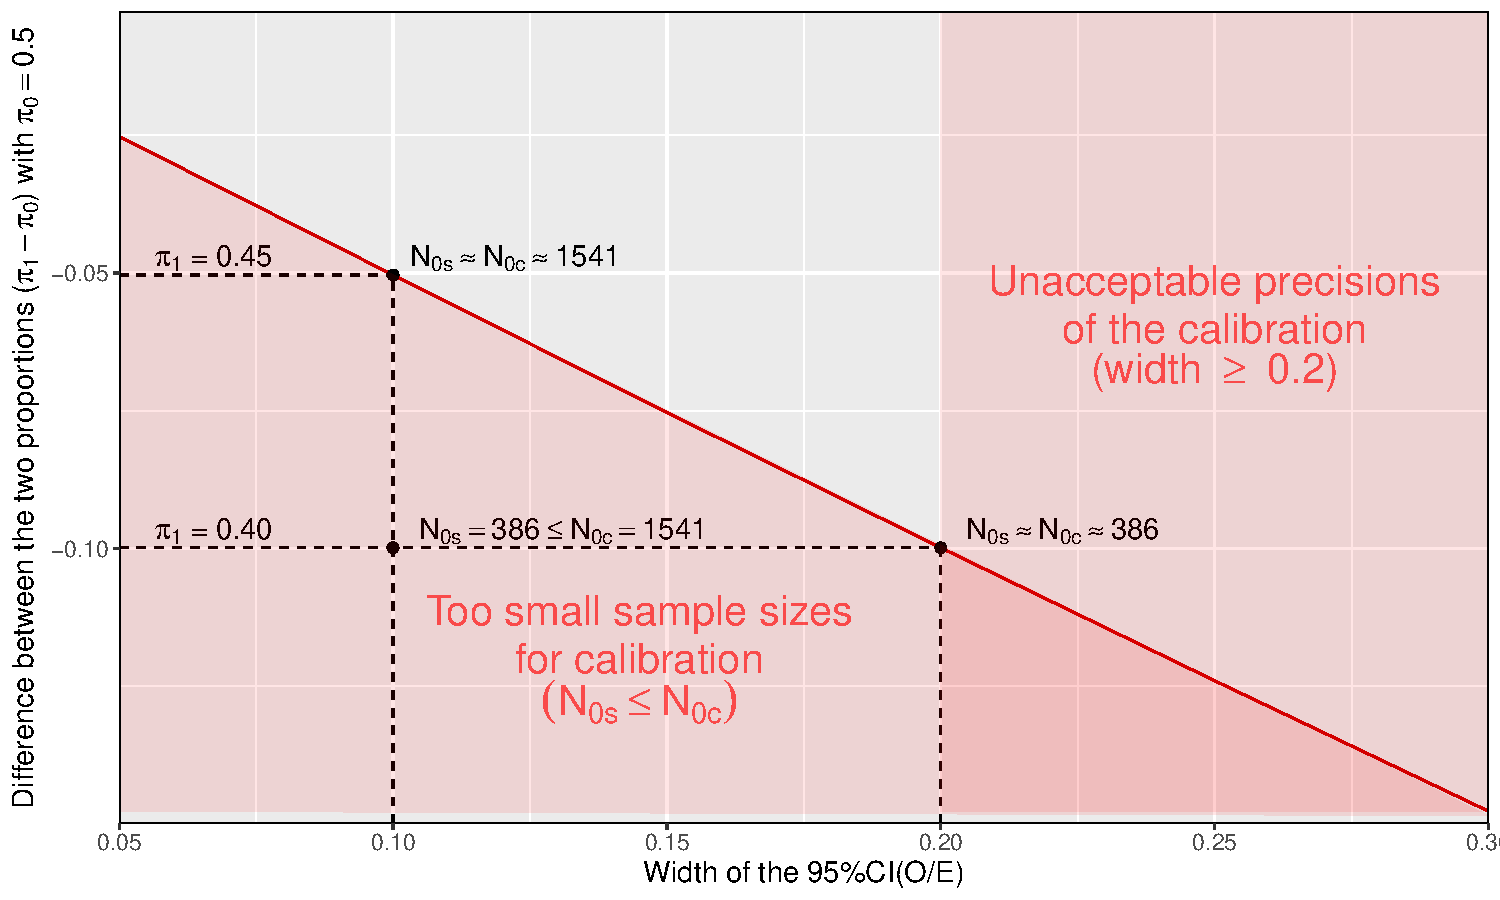
\includegraphics[width=12cm,  keepaspectratio]{figures/ggp3.pdf}
} }

\end{document}


